After observing that 20$\mu$m cryosections of embryonic mouse brain became transparent in the hybridization buffer used for \emph{in situ} hybridization, we found that a component of the buffer, formamide, could clear thick tissue samples.
Here, we demonstrate the versatility of our method, named \emph{Clear\textsuperscript{T}} for neuronal and non-neuronal tissue, and compare its clarity, rapidity, and tissue expansion/shrinkage to existing clearing methods.

Intact embryos, embryonic and postnatal dissected heads, brains, and thick (up to 1000$\mu$m) brain sections, were fixed and sequentially immersed in graded concentrations of formamide (Table~\ref{table:cleartresults}A, Figure~\ref{ClearTFig1}A).

%\begin{landscape}
\begin{table}[hbtp]
\begin{center}
\caption[Clearing Procedures for \emph{Clear\textsuperscript{T}}]{Clearing protocol for various sample types using \emph{Clear\textsuperscript{T}}. Time in final buffer can be determined by visual inspection for desired transparency. O/N=overnight.}
\label{table:cleartresults}
\begin{tabular}{ccccc}
 & \begin{tabular}[c]{@{}c@{}}Whole embryos\\ or heads\end{tabular} & \begin{tabular}[c]{@{}c@{}}Whole dissected\\ brains (E16-P11)\end{tabular} & \begin{tabular}[c]{@{}c@{}}Half embryonic\\ brains\end{tabular} & \begin{tabular}[c]{@{}c@{}}Sections\\ (200-1000$\mu$m)\end{tabular} \\ \hline
20\% formamide & 30 minutes & 30 minutes & 30 minutes & 5 minutes \\
40\% formamide & 30 minutes & 30 minutes & 30 minutes & 5 minutes \\
80\% formamide & 2 hours & 2 hours & 2 hours & 5 minutes \\
95\% formamide & 30 minutes & 30 minutes & 30 minutes & 5 minutes \\
95\% formamide & \begin{tabular}[c]{@{}c@{}}5-16 hours; E11-E15, \\ respectively\end{tabular} & O/N-2 days & 4 hours & 15 minutes
\end{tabular}
\end{center}
\end{table}

\begin{table}[hbtp]
\begin{center}
\caption[Clearing procedures for \emph{Clear\textsuperscript{T2}}]{Clearing protocol for various sample types using \emph{Clear\textsuperscript{T2}}. Time in final buffer can be determined by visual inspection for desired transparency.}
\label{table:cleart2results}
\begin{tabular}{ccc}
 & \begin{tabular}[c]{@{}c@{}}Embryonic heads\\ or brains\end{tabular} & \begin{tabular}[c]{@{}c@{}}Sections \\ (200-1000$\mu$m)\end{tabular} \\ \hline
25\% formamide/10\% PEG & 1 hour & 10 minutes \\
50\% formamide/20\% PEG & 1 hour & 5 minutes \\
50\% formamide/20\% PEG & \begin{tabular}[c]{@{}c@{}}5-16 hours; E11-E15,\\ respectively\end{tabular} & 15-60 minutes
\end{tabular}
\end{center}
\end{table}
%\end{landscape}

The \emph{Clear\textsuperscript{T}} procedure rendered embryonic brains as transparent as with Sca\emph{l}eA2, but did so significantly faster (1 day versus 14 days) (Figure~\ref{ClearTFig1}B).
Completely cleared postnatal day 0 (P0) brain sections were similar to their original size (before clearing=1.0$\pm$0 versus \emph{Clear\textsuperscript{T}}=1.04$\pm$0.02, not significant, n=6 sections) (Figure~\ref{ClearTFig1}C).
Even after prolonged treatment with \emph{Clear\textsuperscript{T}}, sample volume only increased slightly, significantly less than in Sca\emph{l}eA2 [1 day, \emph{Clear\textsuperscript{T}}=1.33$\pm$0.09 versus Sca\emph{l}eA2=1.81$\pm$0.05, P<0.01; 2 days, \emph{Clear\textsuperscript{T}}=1.27$\pm$0.09 versus Sca\emph{l}eA2=1.83$\pm$0.06, P<0.01, n=5 (\emph{Clear\textsuperscript{T}}), 4 (Sca\emph{l}eA2) sections] (Figure~\ref{ClearTSFig1}).
Although formamide is not harmful to tissue in the short term, it is unsuitable for long-term tissue storage.
Therefore, we transferred samples treated with \emph{Clear\textsuperscript{T}} into PBS, where they became opaque within 30 minutes and could be safely stored for at least 1 month (Figure~\ref{ClearTFig1}D).

\begin{figure}[hbtp]
\begin{center}
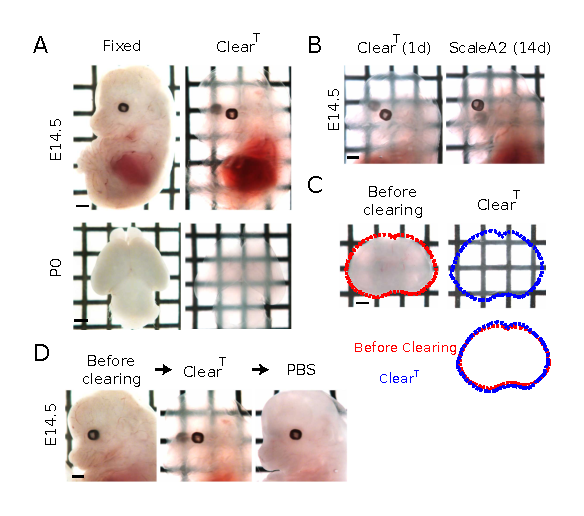
\includegraphics{Figures/ClearT_Fig1}
\caption[Rapid tissue clearing with \emph{Clear\textsuperscript{T}}.]
{Rapid tissue clearing with \emph{Clear\textsuperscript{T}}.
A) Fixed whole embryos (E14.5) and dissected postnatal brains (P0) were cleared overnight.
The grid is visible through tissue cleared by \emph{Clear\textsuperscript{T}}.
B) E14.5 embryos cleared with \emph{Clear\textsuperscript{T}} or Sca\emph{l}eA2 reach full transparency in 1 day or 14 days,
respectively.
C) \emph{Clear\textsuperscript{T}} does not lead to volume changes.
P0 sections (800$\mu$m), surface area measured: pre-cleared, red line; ClearT, blue line.
D) Clearing is reversible with PBS (30 minutes).
Scale bars: 1 mm.
}
\label{ClearTFig1}
\end{center}
\end{figure}

\begin{figure}[hbtp]
\begin{center}
\includegraphics{Figures/ClearT_SFig1}
\caption[Volume changes are minimal after tissue is incubated in \emph{Clear\textsuperscript{T}} and \emph{Clear\textsuperscript{T2}}.]
{Volume changes are minimal after tissue is incubated in \emph{Clear\textsuperscript{T}} and \emph{Clear\textsuperscript{T2}}.
Quantification of size changes of 800mm sections of P0 brain in \emph{Clear\textsuperscript{T}}, \emph{Clear\textsuperscript{T2}} and Sca\emph{l}eA2, after incubation in each solution for 1-2 days.
Surface area was significantly increased after treatment with Sca\emph{l}eA2 compared with \emph{Clear\textsuperscript{T}} and \emph{Clear\textsuperscript{T2}}.
Data are expressed as mean $\pm$ s.e.m.
*=P<0.01, one-way ANOVA followed by Tukey's post hoc test; n=5 (\emph{Clear\textsuperscript{T}}), n=6 (\emph{Clear\textsuperscript{T2}}), n=4 (Sca\emph{l}eA2) sections.
}
\label{ClearTSFig1}
\end{center}
\end{figure}
